% %% %%%%%%%%%%%%%%%%%%%%%%%%%%%%%%%%%%%%%%%%%%%%%%%%%%%%%%%%%%
% steps.tex
%
% Author:  Mauricio Matamoros
% License: MIT
%
% %% %%%%%%%%%%%%%%%%%%%%%%%%%%%%%%%%%%%%%%%%%%%%%%%%%%%%%%%%%%

%!TEX root = ../practica.tex
%!TEX root = ../references.bib

\section{Instrucciones}%
\label{sec:instructions}
\begin{enumerate}[noitemsep]
	\item Configure su entorno de desarrollo tomando siguiendo los pasos de la \Cref{sec:step1}.
	\item Descargue y configure buildroot como se describe en las \Cref{sec:step2,sec:step3}.
	\item Siguiendo los pasos de la \Cref{sec:step4} modifique el sistema de archivos de la distro embebida.
	\item Compile el kernel y genere la imagen de sistema tal como explica la \Cref{sec:step5}
 	\item Grabe la imagen generada en la memoria microSD y pruebe el sistema operativo embebido en la Raspberry Pi de acuerdo con las instrucciones de la \Cref{sec:step6}
 	\item Por último, realice los experimentos propuestos en la \cref{sec:experiments}.
 	% y con los resultados obtenidos responda el cuestionario de la \cref{sec:questionnaire}.
\end{enumerate}

% %% %%%%%%%%%%%%%%%%%%%%%%%%%%%%%%%%%%%%%%%%%%%%%%%%%%%%%%%%%%
% step-1.tex
%
% Author:  Mauricio Matamoros
% License: MIT
%
% %% %%%%%%%%%%%%%%%%%%%%%%%%%%%%%%%%%%%%%%%%%%%%%%%%%%%%%%%%%%
%!TEX root = ../practica.tex
%!TEX root = ../references.bib

% CHKTEX-FILE 1
% CHKTEX-FILE 13
% CHKTEX-FILE 46

\subsection{Implementación un controlador On/Off}%
\label{sec:step-1}

Alambre cuidadosamente los circuitos de las prácticas \href{https://github.com/kyordhel/FSEm/tree/master/practica06}{6} y \href{https://github.com/kyordhel/FSEm/tree/master/practica07}{7} para crear un circuito AC-DC optoacoplado completo para control cerrado de temperatura usando un foco incandescente operado con un LM35 y un circuito de variación de fase mediante detección de cruce por cero.
El circuito completo alambrado debe verse como el de la \Cref{fig:circuit-full}.

\medskip

\begin{importantbox}{\large Importante}
	\begin{center}
		Asegúrese de verificar con un multímetro que el circuito de AC está debidamente aislado y que no se tienen valores mayores a 5V en el segmento de DC.
		De otro modo podría quemar su Arduino y su Raspberry Pi.
	\end{center}
\end{importantbox}

\medskip

\begin{figure}
	\centering
	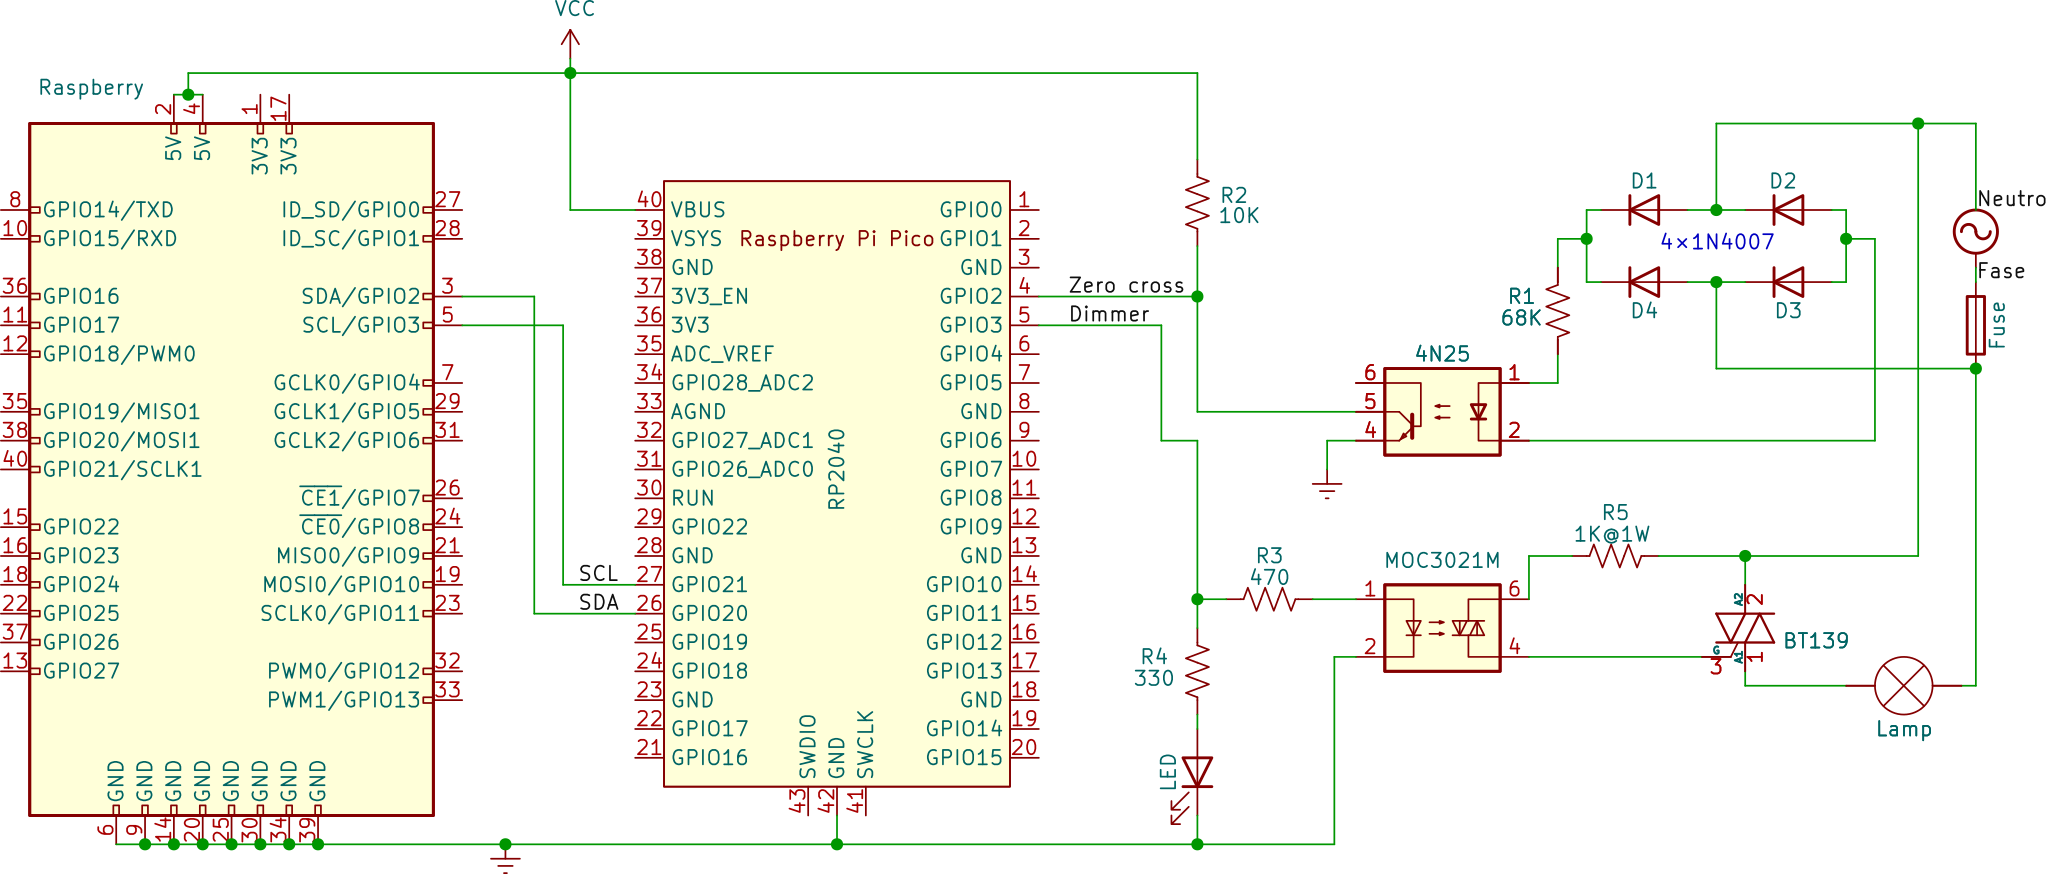
\includegraphics[width=0.85\linewidth,height=6cm,keepaspectratio]{img/circuit-full.png}
	\caption{Circuito AC-DC optoacoplado completo para control cerrado de temperatura.}%
	\label{fig:circuit-full}
\end{figure}

De acuerdo con el alambrado de la \Cref{fig:circuit-full}, el Arduino ha de realizar tres funciones:
\begin{enumerate*}[label=\roman*\rpar]
	\item digitalización del valor de temperatura analógico sensado por el LM35,
	\item la detección del cruce por cero de la onda sinusoidal de la línea eléctrica,
	y
	\item la modulación de potencia del foco incandescente mediante variación de fase ajustada por el retardo en el disparo del TRIAC.
\end{enumerate*}
Al igual que en las prácticas anteriores, el Arduino estará configurado como dispositivo esclavo y estas operaciones estarán al servicio del dispositivo maestro: la Raspberry Pi.
Así, una operación de lectura proporcionará al dispositivo maestro la temperatura sensada, mientras que una operación de escritura enviará la potencia con la que encenderá el foco como un valor flotante entre 0 y 100, quedando a cargo del Arduino el cálculo de la variación de fase y la sincronización de las operaciones de hardware.

\paragraph{Nota:} La implementación del código del Arduino se deja a cargo del estudiante.

\medskip

Se puede proceder entonces a revisar el código de control que se ejecutará en la Raspberry Pi.
En este caso se implementará un controlador On/Off tal como se describe en la \Cref{sec:control-onoff}.

Lo primero es incluir los paquetes necesarios y proveer cuatro parámetros importantes:
\begin{enumerate*}[label=\arabic*\rpar]
	\item la dirección del dispositivo esclavo,
	\item la temperatura deseada,
	\item el umbral o valor de encendido,
	y
	\item el umbral o valor de apagado
\end{enumerate*}
tal como se muestra en el \Cref{lst:controller-code-params}.

\begin{minipage}{\linewidth}%
\lstinputlisting[%
	language=python,
	caption={\texttt{controller-on-off.py:9--20} --- Parámetros},
	label={lst:controller-code-params},
	firstline=9,
	lastline=20]{src/controller-on-off.py}
\end{minipage}

El controlador con los parámetros descritos anteriormente requerirá de dos funciones auxiliares: \emph{readTemperature} (véase \Cref{lst:controller-code-read}) y \emph{writePower} (véase \Cref{lst:controller-code-write}).
La primer función corresponde a una operación de lectura en la cual el Arduino proporcionará la temperatura registrada por el sensor en grados centígrados codificado como un valor flotante (4 bytes en little endian).
La segunda función es una operación de escritura en la cual la Raspberry Pi proporcionará al arduino el factor de potencia de 0 a 100 codificada como un valor flotante (4 bytes en little endian).

\begin{minipage}{\linewidth}%
\lstinputlisting[%
	language=python,
	caption={\texttt{controller-on-off.py:26--36} --- Función \emph{readTemperature}},
	label={lst:controller-code-read},
	firstline=26,
	lastline=36]{src/controller-on-off.py}
\end{minipage}

\begin{minipage}{\linewidth}%
\lstinputlisting[%
	language=python,
	caption={\texttt{controller-on-off.py:38--45} --- Función \emph{writePower}},
	label={lst:controller-code-write},
	firstline=38,
	lastline=45]{src/controller-on-off.py}
\end{minipage}

Por último queda revisar la implementación del controlador mostrada en el \Cref{lst:controller-onoff-code}.
El control de temperatura se ejecuta en un bucle infinito de tres partes dentro de la función principal \emph{main}.
\begin{enumerate*}[label=\arabic*\rpar]
	\item Primero se lee la temperatura en °C del arduino,
	\item después esta se compara con los umbrales.
	Si la temperatura es menor al valor de encendido la lámpara se enciende a máxima potencia y permanecerá encendida hasta que se supera el valor de apagado.
	Por último,
	\item el controlador entra en un estado de espera (1 segundo) donde no se realiza ninguna acción.
\end{enumerate*}
En cualquier otro caso no se hace nada.

\begin{minipage}{\linewidth}%
\lstinputlisting[%
	language=python,
	caption={\texttt{controller-on-off.py:47--67} --- Función \emph{main}},
	label={lst:controller-onoff-code},
	linerange={47-47,51-52,54-55,57-67} %CHKTEX 8
	]{src/controller-on-off.py}
\end{minipage}
% %% %%%%%%%%%%%%%%%%%%%%%%%%%%%%%%%%%%%%%%%%%%%%%%%%%%%%%%%%%%
% step-2.tex
%
% Author:  Mauricio Matamoros
% License: MIT
%
% %% %%%%%%%%%%%%%%%%%%%%%%%%%%%%%%%%%%%%%%%%%%%%%%%%%%%%%%%%%%

%!TEX root = ../main.tex
%!TEX root = ../references.bib

\subsection{Paso 2: Led parpadeante}%
\label{sec:step2}
El código mostrado en \Cref{src:blink} muestra cómo se haría parpadear un LED mediante tiempos de espera o \emph{sleeps} utilizando la Raspberry Pi.

\smallskip
\lstinputlisting[%
	language=Python,
	linerange={18-40}, % chktex 8
	caption={\texttt{blink.py}},
	label={src:blink}
]{src/blink.py}
\smallskip

Estudie el código y véalo en funcionamiento, ejecutándolo de la siguiente manera:
\begin{Verbatim}[fontsize=\footnotesize]
./blink.py
\end{Verbatim}

% %% %%%%%%%%%%%%%%%%%%%%%%%%%%%%%%%%%%%%%%%%%%%%%%%%%%%%%%%%%%
% step-3.tex
%
% Author:  Mauricio Matamoros
% License: MIT
%
% %% %%%%%%%%%%%%%%%%%%%%%%%%%%%%%%%%%%%%%%%%%%%%%%%%%%%%%%%%%%
%!TEX root = ../practica.tex
%!TEX root = ../references.bib

% CHKTEX-FILE 1
% CHKTEX-FILE 13
% CHKTEX-FILE 46
\subsection{Paso 3: Control en lazo abierto de la potencia de una carga resistiva}%
\label{sec:step3}
Antes de proceder, verifique conexiones con un multímetro en busca de corto circuitos.
En particular verifique que los circuitos de AC y DC funcionan de manera independiente y que existe una impedancia infinita entre pines optoacoplados.

Con la Raspberry Pi configurada, basta con generar los dos programas para transferir la potencia de salida deseada de la Raspberry Pi al RP2040 que se encargará cortar el flujo de corriente en el instante correcto para obtener la potencia deseada.

Primero, es necesario configurar al RP2040 como dispositivo esclavo e inicializar el bus \IIC, tal como se muestra en el \Cref{lst:rp2040-test-i2c-setup}.
Las comunicaciones via \IIC son síncronas, lo que simplifica enormemente el diseño del programa.

\lstinputlisting[%
	language=Python,
	caption={\texttt{rp2040-test-i2c.py:23} --- Dirección asignada al dispositivo esclavo},
	label={lst:rp2040-test-i2c-setup},
	linerange=23-23]{src/rp2040-test-i2c.py} %CHKTEX 8

Tanto el envío como la recepción de datos se realizan byte por byte, por lo que es necesario convertir la potencia (\emph{float}) en un arreglo de bytes que pueda ser transmitido.
Para esta opreación se utilizará la librería \texttt{ustruct} que empaquetará y desempaquetará flotantes (\emph{float}) en listas de 4 bytes que pueden ser enviados o recibidos via \IIC de manera análoga a como se muestra en los \Cref{lst:rpi-code-i2c-read,lst:rpi-code-i2c-write}


Del lado de la Raspberry Pi, primero ha inicializarse el bus \IIC y posteriormente se realizarán las lecturas en un poleo o bucle infinito, cada una de las cuales se irá almacenando en un archivo bitácora.
La inicialización del bus requiere de una simple línea (véase \Cref{lst:rpi-code-i2c-setup}).

\lstinputlisting[%
	language=Python,
	caption={\texttt{raspberry-code-i2c.py:18} --- Configuración del bus \IIC},
	label={lst:rpi-code-i2c-setup},
	linerange=18-18]{src/raspberry-code-i2c.py} %CHKTEX 8

La conversión de un arreglo de bytes a punto flotante en Python no es inmediata.
Para esta opreación se utilizará la librería \texttt{struct} que empaquetará y desempaquetará flotantes (\emph{float}) en listas de 4 bytes que pueden ser enviados o recibidos del RP2040 via \IIC tal como se muestra en los \Cref{lst:rpi-code-i2c-read,lst:rpi-code-i2c-write}

\lstinputlisting[%
	language=Python,
	caption={\texttt{raspberry-code-i2c.py:36--43} --- Escritura de flotantes en el bus \IIC},
	label={lst:rpi-code-i2c-write},
	linerange=36-43]{src/raspberry-code-i2c.py} %CHKTEX 8

\lstinputlisting[%
	language=Python,
	caption={\texttt{raspberry-code-i2c.py:20--34} --- Lectura de flotantes del bus \IIC},
	label={lst:rpi-code-i2c-read},
	linerange=20-34]{src/raspberry-code-i2c.py} %CHKTEX 8


El resto del programa es trivial, pues consiste sólo en solicitar al usuario un valor de potencia y enviarlo al RP2040.

Por conveniencia, los códigos completos de los programas de ejemplo se encuentran en los \Cref{sec:appendix1,sec:appendix2,sec:appendix3,sec:appendix4}.

% %% %%%%%%%%%%%%%%%%%%%%%%%%%%%%%%%%%%%%%%%%%%%%%%%%%%%%%%%%%%
% step-4.tex
%
% Author:  Mauricio Matamoros
% License: MIT
%
% %% %%%%%%%%%%%%%%%%%%%%%%%%%%%%%%%%%%%%%%%%%%%%%%%%%%%%%%%%%%

%!TEX root = ../practica.tex
%!TEX root = ../references.bib

% CHKTEX-FILE 1
% CHKTEX-FILE 13
% CHKTEX-FILE 46

\subsection{Paso 4: Bitácora de temperatura via \IIC}%
\label{sec:step4}

Con la Raspberry Pi configurada, basta con generar los dos programas para transferir las temperaturas registradas en el Arduino a la Raspberry Pi que se encargará de almacenar esta información en un archivo o bitácora.

Primero, es necesario configurar al Arduino como dispositivo esclavo e inicializar el bus \IIC, tal como se muestra en los \Cref{lst:arduino-code-i2c-def,lst:arduino-code-i2c-setup}.
Las comunicaciones via \IIC son asíncronas, por lo que se requerirá almacenar la temperatura en una variable global que será leída por la función que atenderá las peticiones de datos del dispositivo maestro (la Raspberry Pi).

\lstinputlisting[%
	language=C,
	caption={\texttt{arduino-code-i2c.cpp:16} --- Dirección asignada al dispositivo esclavo},
	label={lst:arduino-code-i2c-def},
	firstline=16,
	lastline=16]{src/arduino-code-i2c.cpp}

\lstinputlisting[%
	language=C,
	caption={\texttt{arduino-code-i2c.cpp:37--42} --- Configuración del bus \IIC y funciones de control},
	label={lst:arduino-code-i2c-setup},
	firstline=37,
	lastline=42]{src/arduino-code-i2c.cpp}

El envío de datos se realiza byte por byte, por lo que es necesario convertir la medición de temperatura (\emph{float}) en un arreglo de bytes que pueda ser transmitido.
Esto se hace en la función \texttt{i2c\_request\_handler} con una llamada a \texttt{Wire.write} tal como se ilustra en el \Cref{lst:arduino-code-i2c-reqh}.

\lstinputlisting[%
	language=C,
	caption={\texttt{arduino-code-i2c.cpp:58--60} --- Envío asíncrono de datos},
	label={lst:arduino-code-i2c-reqh},
	firstline=56,
	lastline=58]{src/arduino-code-i2c.cpp}

Del lado de la Raspberry Pi, primero ha inicializarse el bus \IIC mediante el uso de la librería \texttt{smbus}\footnotemark y posteriormente se realizarán las lecturas en un poleo o bucle infinito, cada una de las cuales se irá almacenando en un archivo bitácora.
La inicialización del bus requiere de una simple línea (véase \Cref{lst:rpi-code-i2c-setup}).
\footnotetext{La implementación de la práctica utiliza \texttt{smbus2} que es una reimplementación codificada exclusivamente en Python de la librería \texttt{smbus} que es un \emph{wrapper} de la \emph{smbuslib} de C.}

\lstinputlisting[%
	language=Python,
	caption={\texttt{raspberry-code-i2c.py:26} --- Configuración del bus \IIC},
	label={lst:rpi-code-i2c-setup},
	linerange={9-10,19-21}% CHKTEX 8
	]{src/raspberry-code-i2c.py}

La conversión de un arreglo de bytes a punto flotante en Python no es inmediata.
Para esta opreación se utilizará la librería \texttt{struct} (véase \Cref{lst:rpi-code-i2c-setup}) que tomará los cuatro paquetes de 1 byte recibidos vía \IIC del Arduino y los convertira en un \emph{float}, como se muestra en el \Cref{lst:rpi-code-i2c-read}.
Nótese el símbolo $<$ (menor qué) a la izquierda del especificador de formato $f$, el cual se utiliza para definir el endianness de la transmisión de la información.

\lstinputlisting[%
	language=Python,
	caption={\texttt{raspberry-code-i2c.py:28--35} --- Lectura de flotantes del bus \IIC},
	label={lst:rpi-code-i2c-read},
	linerange={23-35} %CHKTEX 8
	]{src/raspberry-code-i2c.py}

El resto del programa es trivial, pues consiste sólo en la escritura del \emph{timestamp UNIX} y el valor de temperatura registrado en un archivo de texto y la lectura de datos del arduino cada segundo.

Por conveniencia, los códigos completos de los programas de ejemplo se encuentran en los \Cref{sec:appendix1,sec:appendix2,sec:appendix3}.

% %% %%%%%%%%%%%%%%%%%%%%%%%%%%%%%%%%%%%%%%%%%%%%%%%%%%%%%%%%%%
% step-4.tex
%
% Author:  Mauricio Matamoros
% License: MIT
%
% %% %%%%%%%%%%%%%%%%%%%%%%%%%%%%%%%%%%%%%%%%%%%%%%%%%%%%%%%%%%

%!TEX root = ../practica.tex
%!TEX root = ../references.bib

% CHKTEX-FILE 1
% CHKTEX-FILE 13
% CHKTEX-FILE 46

\subsection{Paso 5: Temperatura del RP2040}%
\label{sec:step5}

La \cref{eqn:v-to-temp} tiene un problema fundamental: un convertidor ADC entrega valores discretos enteros que corresponden de forma proporcional y lineal al voltaje sensado entre $V_\text{Ref-}$ y $V_\text{Ref+}$.
En el caso del RP2040 $V_\text{Ref-} = \text{\textsc{Gnd}} = 0\text{V}$ y $V_\text{Ref+} = \text{\textsc{Vcc}} = 3.3\text{V}$ y, dado que la precisión del ADC es de 12bits, los valores registrados estarrían entre cero y $2^{12}-1 = 4095$.
Sin embargo, MicroPython ofrece el método \code{read_u16()} de las instancias de \code{ADC} que provee un entero no signado de 16 bits.
Así, las conversiones tendrán que tomar en cuenta un rango entre 0 y 65535.

Con esto en mente y considerando que $v = \frac{3.3V}{65535}x$, se puede reemplazar $v$ por $x$ en la \cref{eqn:v-to-temp} para obtener una fórmula de conversión directa del valor reportado del ADC a un valor de temperatura.

\noindent
Así, la \cref{eqn:v-to-temp} quedaría como:

\begin{align*}%
	\label{eqn:adc-to-temp}
	T &=%
		\Bigg( \frac{-1}{1.721\frac{\text{mV}}{\text{°C}}} \Bigg)
		\Bigg( \frac{3.3\text{V}}{65535} \cdot x \Bigg) +
		437.23\text{°C} \\
%
	  &=
		\Bigg( \frac{-1}{1.721\frac{\text{mV}}{\text{°C}}} \Bigg)
		\Bigg( \frac{3300\text{mV}}{65535} \cdot x \Bigg) +
		437.23\text{°C} \\
%
	  &=
		\frac{
			-3300\cancel{\text{mV}}
		}{
			65535 \times 1.721\frac{\cancel{\text{mV}}}{\text{°C}}
		}
		\cdot x +
		437.23\text{°C} \\
%
	  &=
		\frac{
			-3300
		}{
			112785.74\frac{1}{\text{°C}}
		}
		\cdot x +
		437.23\text{°C} \\
\end{align*}

\noindent
Lo que finalmente produce la ecuación:

\begin{equation}%
	\label{eqn:adc-to-temp}
	T = -29259\times10^{-6}x + 437.23
\end{equation}

\noindent
Esta ley se refleja en el código presentado en \cref{lst:temp}.

\medskip{}

\noindent
Ingrese el siguiente código en el editor de Thonny y ejecútelo

\lstinputlisting[%
	language=Python,
	caption={\texttt{temp.py}: --- Temperatura del RP2040},
	label={lst:temp},
	firstline=11
]{src/temp.py}


El \cref{lst:temp} configura primero el ADC para leer del canal 4 (sensor interno de temperatura) y luego define un bucle infinito con la cláusula \code{while} dentro del cual
\begin{enumerate*}[label=\roman*\rpar]
	\item se lee el valor del convertidor A/D,
	\item se convierte el valor sensado a temperatura en grados celcius
	\item se imprime la temperatura
	y, finalmente,
	\item se espera durante un segundo.
\end{enumerate*}

Por conveniencia, los códigos completos de los programas de ejemplo se encuentran en el \Cref{sec:appendix3}.

% %% %%%%%%%%%%%%%%%%%%%%%%%%%%%%%%%%%%%%%%%%%%%%%%%%%%%%%%%%%%
% step-6.tex
%
% Author:  Mauricio Matamoros
% License: MIT
%
% %% %%%%%%%%%%%%%%%%%%%%%%%%%%%%%%%%%%%%%%%%%%%%%%%%%%%%%%%%%%

%!TEX root = ../practica.tex
%!TEX root = ../references.bib

% CHKTEX-FILE 1
% CHKTEX-FILE 13
% CHKTEX-FILE 46

\subsection{Paso 6: Grabación y prueba}%
\label{sec:step6}
Una vez que el sistema termine de compilar, encontrará la imagen generada \texttt{.img} dentro del directorio \texttt{output/images} de \emph{buldroot}.
Notará que el archivo de imagen no pesa más de 300MB.
¡Así de pequeño es su sistema operativo embebido!

Proceda a grabar la imagen generada en una memoria microSD utilizando \href{https://etcher.balena.io/}{Balena Etcher} de la misma forma que ha grabado otras imágenes.
Alternativamente puede grabar la imagen utilizando \texttt{dd} si conoce la ruta de la misma en su sistema con el comando:

\begin{Verbatim}[gobble=1]
	# dd if=output/images/sdcard.img of=/dev/<memoriaSD> bs=10M status=progress
\end{Verbatim}

\noindent
La grabación no debería tomar más que unos segundos.

% \begin{wrapfigure}{r}{0.4\textwidth}
% 	\centering
% 	\includegraphics[width=0.38\textwidth]{img/system-running.jpg}
% \end{wrapfigure}
\begin{figure}
	\centering
	\includegraphics[width=0.8\textwidth,height=7cm,keepaspectratio]{img/system-running.jpg}
	\caption{Sistema embebido en ejecución con logotipo personalizado}%
	\label{fig:system-running}
\end{figure}
\medskip{}

Terminada la grabación, inserte la memoria microSD en la Raspberry Pi y observe el proceso de arranque, tendría que ver una pantalla similar a la de la~\Cref{fig:system-running}.
Cuando se lo solicite, inicie sesión con el usuario \texttt{pi} y la contraseña \texttt{raspberry}.


Conecte el display al puerto \IIC{} (pines 3 y 5 del puerto o GPIO2 y GPIO3 en BCM) y ejecute el comando de detección de dispositivos

\begin{Verbatim}[gobble=1]
	$ i2cdetect -y 1
\end{Verbatim}

\noindent
tendría que ver una salida como la siguiente:

\begin{Verbatim}[gobble=1]
	$ i2cdetect -y 1
	     0  1  2  3  4  5  6  7  8  9  a  b  c  d  e  f
	00:          -- -- -- -- -- -- -- -- -- -- -- -- --
	10: -- -- -- -- -- -- -- -- -- -- -- -- -- -- -- --
	20: -- -- -- -- -- -- -- 27 -- -- -- -- -- -- -- --
	30: -- -- -- -- -- -- -- -- -- -- -- -- -- -- -- --
	40: -- -- -- -- -- -- -- -- -- -- -- -- -- -- -- --
	50: -- -- -- -- -- -- -- -- -- -- -- -- -- -- -- --
	60: -- -- -- -- -- -- -- -- -- -- -- -- -- -- -- --
	70: -- -- -- -- -- -- -- --
\end{Verbatim}

